%Author Alex Clemmer
%CS 3130 Eng Stats Prob
%Assignment 7:
\documentclass[a4paper]{article}
\usepackage[pdftex]{graphicx}
\usepackage{fancyvrb}
\usepackage{multirow}
\usepackage{amssymb}
\usepackage{amsmath}
\usepackage{haldefs}
\usepackage{fullpage}
\addtolength{\oddsidemargin}{-.05in}
	\addtolength{\evensidemargin}{-.05in}
	\addtolength{\textwidth}{.25in}

	\addtolength{\textheight}{.25in}

\begin{document}

\section*{Assignment 7}
Alex Clemmer\\
CS 3100 \\
Student number: u0458675

\subsection*{Problem 1:} 

\paragraph{(a)} The value I chose for $w$ is $\texttt{aaaaaabbbbbbaaaaaabbbbbb}$.

\paragraph{(b)} The value I chose for $i$ is $\texttt{2}$.

\paragraph{(c)} For $L= \{ww : w \in \{a,b\}^*\}$ and $w = a^n b^n a^n b^n$, there is absolutely no way that we could pick some part of $w$ such that pumping it would give us a string inside $L$. Consider $w=uvxyz$. We can only pump $v$ and $y$, so no matter what we choose for each division of $w$, we will always end up doubling either part of the string, and not another part of the string such that it excludes the string from $L$.

The reason this is that doubling only two of the composing variables will allow us to either double only 2 of the 4 variables (e.g., $w = a^n b^i a^i b^n : i \neq n$), or else we end up doubling two types of character at once, giving us too many characters to be in $L$, (e.g., $w = a^n b^n a^n b^n a^n b^n$).

Here are some examples: if $v= aaa$ from the second set of $a$'s, and $y=bbb$ from the second set of $b$'s, then pumping gives us $w = a^n b^i a^i b^n : i \neq n$, and thus it is not in $L$. If $v = a^n b^n$ and $y= a^n b^n$, pumping gives us $w= a^n b^n a^n b^n  a^n b^n  a^n b^n$, which is also not in $L$. And so it goes.

\subsection*{Problem 2:} 

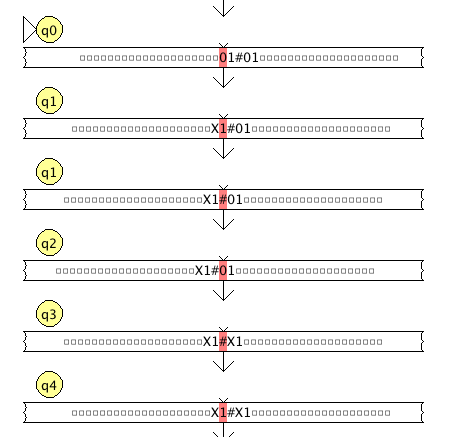
\includegraphics[scale=0.50]{p2_trace.png}

\subsection*{Problem 3:}

We freeze in two places. First, on step 2: \\

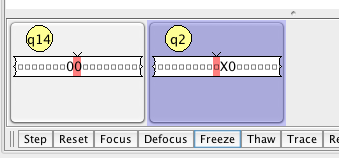
\includegraphics[scale=0.50]{freeze_step_2.png} \\

...and second, on step 3: \\

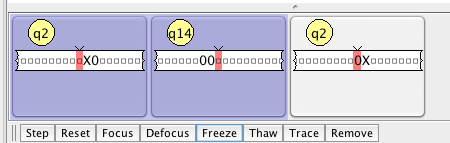
\includegraphics[scale=0.50]{freeze_step_3.png} \\

And here's the trace: \\

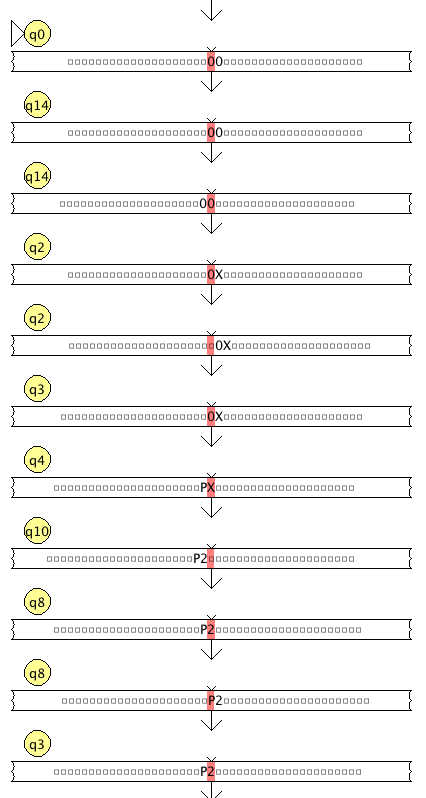
\includegraphics[scale=0.50]{p3_trace.png}

\subsection*{Problem 4:}

This TM accepts all strings with the substring $\texttt{0101}$.

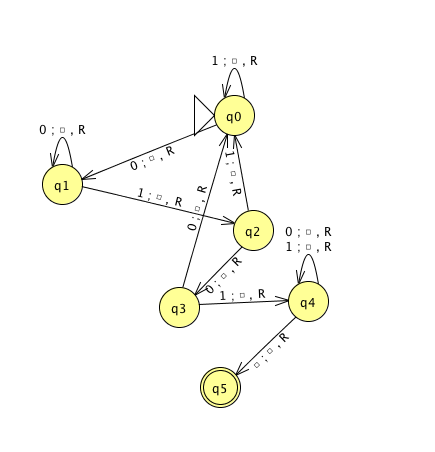
\includegraphics[scale=0.6]{p4_TM.png}

The required test is as follows; there are more tests included, but the one you're looking for is the very last one. \\

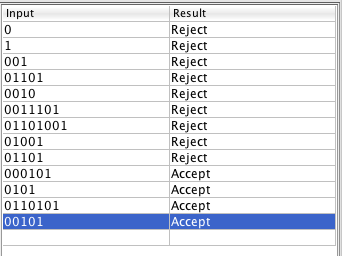
\includegraphics[scale=0.6]{p4_validation.png}

\subsection*{Problem 5:}

The TM and tests are below:

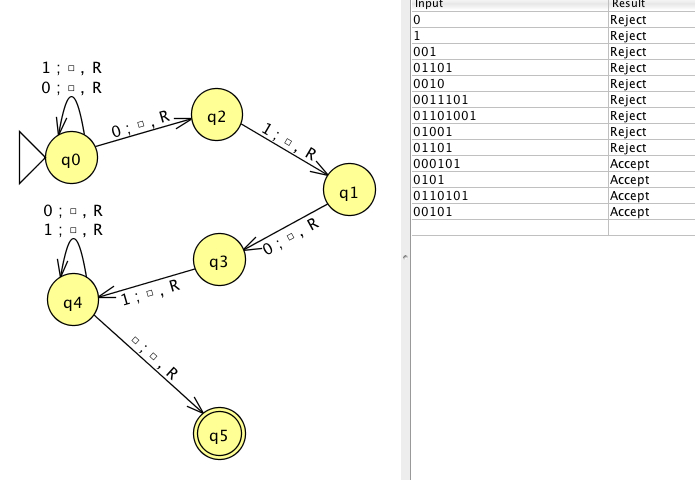
\includegraphics[scale=0.4]{p5_tm_and_trace.png} \\

Below is the picture of all the paths that would lead to rejection (and were thus frozen), along with the one path that would lead to accept. They were frozen at 2nd and 5th steps, respectively. \\

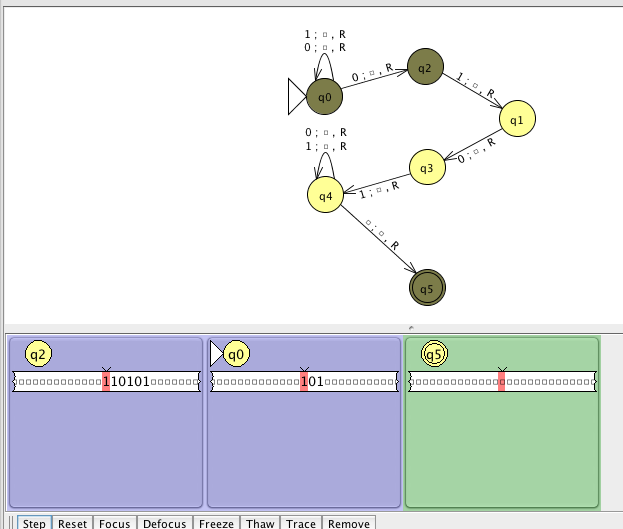
\includegraphics[scale=0.4]{p5_freeze.png} \\

\subsection*{Problem 6:}

\paragraph{(a)} The language $L = \{0^n 1^n | n \ge 0 \}$ is a problem we've faced repeatedly in the course. It is a CFL; since TMs can recognize any CFL, it is clearly recursively enumerable. To recognize this string, we need only one stack, the TM need only count the number of 0s and repeatedly pop the count when it reaches the 1s. At the end, there should be both an empty stack and a consumed string.

It turns out that this language is also recursive. In order to recognize all strings not in $L$, all we need to do is look for every type of string that is $\textit{not}$ in $L$. This rule is not hard in principle, but it does require some careful attention to exceptions and corner cases. You would check, for example, strings where 0 and 1 are not in that order, where there's different numbers of each, where they both occur more than once (e.g., 0101010, rather than $0^n 1^n$), and so on.

Since both the original CFL and its complement can be emulated by a TM, they will always cause the TM to halt, and thus the language again is recursive.

\paragraph{(b)} This is also recursive. Any language representable by a regular expression is a regular language, which can be emulated with a TM. If you're wondering, one example of a regex that fulfills these criteria is $L = (01)^*$, which is recursive, and also has an infinite number of strings. Again, since this is an RL, all the TM needs to do is emulate the FA that describes this regex.

Also, since RLs are closed over the complement operation, all the above will hold for its inverse. Thus, the TM will halt in every case, whether it accepts or not. The language is therefore recursive.

\paragraph{(c)} Recursive. A TM can simulate some arbitrary TM. Since here the stipulation is that the TMs we are accepting also accepts the string $\texttt{0101}$, we know they represent a regular language, and thus will halt for all finite input. Since these TMs represent an RL, they are also closed over inversion, and their complements will thus also halt over any finite. Thus we know that this language is also recursive.

\paragraph{(d)} This language consists essentially of all TMs: any possible TM will either accept, reject, or loop over the string $\texttt{0101}$. The set of all TMs is RE, but it is not recursive, because we do not know that it halts over all elements in the language (and in fact for some, definitely won't). So it's RE but not recursive.

\paragraph{(e)} Both the number of CFGs and regular expressions that have $\texttt{0101}$ are infinite. Important also is that we know that the regular expression is not infinite, as it is representative of a regular language. Also, RLs are invertible, so that part of the equation is for sure recursive.

What is slightly more tricky is the CFG. CFGs are not closed over inversion, so we have no guarantee that the CFGs in this set are recursive. So it's only RE.

\subsection*{Problem 7:}

This problem is actually a lot simpler than it seems. If $P$ will accept only in the event that $M$ accepts $x$, and then $N$ accepts $x$, then $P$ clearly must accept only the strings that both $M$ and $N$ accept. Thus, $L(P) = \{ L(N) \cap L(M) \}$. It's really that simple.


\section*{Extra Credit Questions:}

\subsection*{Problem 8:}

An algorithm is a set of steps designed to solve some problem. Some definitions insist that algorithms halt, and others do not. There are other �invariants� like this, but for most purposes, these small details are not critical; what is critical is that it can generally be represented with some type of machine, and often, which type of machine is equally important.

Some algorithms are deterministic; others are not. For example, some of algorithms are �randomized� (whose randomness is ironically implemented using deterministic algorithms).

The simplest algorithms can be represented by a machine with some finite number of states, and no stacks. That is, the language of the algorithm is enumerable by some Regular Language. The machines that process RLs are FAs, and they have no ability to make new memory: their only memory is their state.

Important to note is that if an algorithm is enumerable by a Regular Language, but is also non-deterministic, it can also be represented by a deterministic machine without simulating states, and almost always with no real massive increase in number of states.

Some algorithms require only a finite number of states, but cannot be represented without at least 1 stack. The language of these algorithms can be derived using Context-Free Grammars.

This might seem like an artificial transition from the simple elegance of a Recursive Language. After all, why a stack? Isn�t that just an arbitrary data structure?

No, it�s not. The point of automata theory is to ask what the minimum required amount of stuff is to calculate some thing, or some type of thing. If we have a machine that can only have a finite number of states, and whose memory is that set of states, then it�s a Regular Language. The next logical machine in that hierarchy is a machine that has the simplest memory possible.

What is the simplest memory possible? A single stack. A list is simple too, but you have to remember the order and protocols for disposal of memory; a stack is easier because you only have access to 1 element, and disposing of it makes way for new memory to be written easily, quickly, and with no overhead after you pop. You can simulate some very simple data structures with a single stack, but there are distinct limitations.

CFGs can be described with a PDA. The main advantage a PDA has is that it can simulate algorithms that have certain types of computation that require itself as an input. For example, for the language $L = {0^n 1^n}$ requires that we count the number of 1s based on the number of 0s that have appeared.

It is here that we begin to see the recursive nature of computation. In this case, to proceed and to look at some algorithm, we need to know something about the computation itself. This case is the simplest recursive relationship an algorithm can have. If you get any more complex, you end up needing two stacks, as we will see.

One important impact of this hierarchy that you can discern given what we�ve established so far is that each higher level can simulate the level below it. That is, an NFA can easily simulate an FA, but going the other direction is tricky. The PDA can simulate an NFA; unfortunately, the NFA cannot simulate the PDA, as it has no ability to write new memory. In other words, these machines form a hierarchy; they are not independent computational models, but rather build on each other.

At this point, one might ask what other resources an algorithm could possibly need. Well, imagine that we wanted to print the number of 1s depending on some variable set a long time ago. If we have only one stack, we could not do this: we can only track the immediate context of our algorithm.

But if we had two stacks, we could (naively) just pop everything to the other stack until we found our variable condition, and then go from there. This subtle difference gives Turing Machines a distinct and substantive advantage over other machine types. Thus algorithms that can be represented by a TM can be a lot more powerful than its predecessors.

One important consequence of this is that algorithms in the TM�s solutions space can actually emulate themselves, which is a novel consequence of these machines. PDAs, NFAs, and DFAs do not have this ability; since TMs can keep track of context throughout a program, they can also thus have algorithms that simulate other algorithms and so on. And this leads to a host of all sorts of problems.

First, and most prominently, given an arbitrary input and an arbitrary machine over an infinite domain, we can�t tell for certain if a TM halts and makes a decision. Consider that to algorithmically decide whether any TM will halt given some input, we must feed it some TM an algorithm that is simulating some other TM simulating an algorithm. If we end up feeding that TM itself as its input, then it can�t ever determine whether it will halt, because if it doesn�t, the answer is no, in which case the answer must become yes, because we have just determined the answer, but then the answer must be no again, and so on. So for every TM, excluding other corner cases, there is at least some inputs that it will not be able to decide on.

This is an important limitation for algorithms, because it means that even given an infinitely powerful machine, there are some algorithms that may not be computed at all. And there are degrees of this: some algorithms halt when you give them an valid input, and may not when you don�t. This sort of algorithm would be Recursively Enumerable, where one that both halts on valid or invalid input would be Recursive.

If this doesn�t seem important, keep in mind that as a joke people will post problems that we know are not decidable to freelance websites like elance, and unsuspecting programmers will still respond. In other words, it pays to know the limitations of your tools, in spite of what other people may tell you.

\subsection*{Problem 9:}

One possible solution is $\texttt{3423}$:

\begin{verbatim}
0    10  0001  0    ->  01000010
010  0   0     010  ->  01000010
\end{verbatim}

\subsection*{Problem 10:}

The solver itself completely rearranged the order of the problem and then came up with a slightly different solution, which was in reverse order of what it really meant.

Given:
\begin{verbatim}
1000  0    0001  10
1     010  0     0
\end{verbatim}

The solution is $\texttt{2342}$ (note that this is reversed):

\begin{verbatim}
0    10  0001  0    ->  01000010
010  0   0     010  ->  01000010
\end{verbatim}

\subsection*{Problem 11:}

I picked one of the simplest puzzles possible:

\begin{verbatim}
2 2
1        00
1000000  0
\end{verbatim}

For which the solution is $\texttt{1222222}$ (note that this is $\textit{not}$ reversed):
\begin{verbatim}
1        00  00  00  00  00  00  ->  1000000000000
1000000  0   0   0   0   0   0   ->  1000000000000
\end{verbatim}

\subsection*{Problem 12:}

I don't know what you mean by "given" equation, so I just played around with it. Linear Diophantine equations are solvable for arbitrarily large $x$ and $y$. This program confirms this for several large $x$ and $y$. This should suffice as an example, although there are other solvable Diophantine equations for large $x$ and $y$. (There are also unsolvable ones, like FLT.)

\subsection*{Problem 13:}

This tells us that decidability is not necessarily dependent on the size of the problem. Rather, there are certain types of problem that, even expressed succinctly, and even given simple features, turn out to be not only undecidable. That is, they are not only difficult, but unable to be computed in the way we traditionally think of computation.

\end{document}